% Version 2016-11-14
% update – 161114 by Ken Arroyo Ohori: made spacing closer to Word template throughout, put proper quotes everywhere, removed spacing that could cause labels to be wrong, added non-breaking and inter-sentence spacing where applicable, removed explicit newlines

\documentclass{isprs}
\usepackage{subfigure}
\usepackage{setspace}
\usepackage{geometry} % added 27-02-2014 Markus Englich
\usepackage{epstopdf}
\usepackage[labelsep=period]{caption}  % added 14-04-2016 Markus Englich - Recommendation by Sebastian Brocks

\geometry{a4paper, top=25mm, left=20mm, right=20mm, bottom=25mm, headsep=10mm, footskip=12mm} % added 27-02-2014 Markus Englich
%\usepackage{enumitem}

%\usepackage{isprs}
%\usepackage[perpage,para,symbol*]{footmisc}

%\renewcommand*{\thefootnote}{\fnsymbol{footnote}}
\captionsetup{justification=centering} % thanks to Niclas Borlin 05-05-2016

\usepackage{listings}
\lstset{basicstyle=\ttfamily\scriptsize,
  showstringspaces=false}

\usepackage{url}

\begin{document}

\title{Building complete free and open source GIS infrastructure for hydrological computing and data publication using GIS.lab and Gisquick platforms}

% KAO: Remove extra spacing
\author{
  M. Landa\textsuperscript{a}, P. Kavka\textsuperscript{b}, L. Strouhal\textsuperscript{b}, J. Cepicky\textsuperscript{c}
}

% KAO: Remove extra newline
\address{
  \textsuperscript{a }Dept.\ of Geomatics, Faculty of Civil Engineering, Czech Technical University in Prague, Czech Republic - martin.landa@fsv.cvut.cz\\
  \textsuperscript{b }Dept.\ of Irrigation, Drainage and Landscape Engineering, Czech Technical University in Prague, Czech Republic - \\
  (petr.kavka, ludek.strouhal)@fsv.cvut.cz\\
  \textsuperscript{c }OpenGeoLabs s.r.o., Prague, Czech Republic - jachym.cepicky@opengeolabs.cz
}

% If the corresponding author is NOT the final author, always add a % space before the subsequent comma, i.e.
% first author name\textsuperscript{a,}\thanks{Corresponding author} , % second author name \textsuperscript{b}, etc.
% thanks to Niclas Borlin 05-05-2016


\commission{}{} %This field is optional.
\workinggroup{} %This field is optional.
\icwg{}   %This field is optional.

% KAO: Use times symbol
\abstract{ Building complete free and open source GIS computing and
  data publication platform can be relatively easy task. This paper
  describes automated deployment of such platform using two open
  source software projects -- GIS.lab and Gisquick. GIS.lab
  (\url{http://web.gislab.io}) is a project for rapid deploying
  complete, centrally managed and horizontally scalable GIS
  infrastructure in local area network, data center or cloud. It
  provides comprehensive set of free geospatial software seamlessly
  integrated into one, easy-to-use system. A platform for GIS
  computing (in our case demonstrated on hydrological modeling)
  requires core components like geoprocessing server, map server, and
  computation engine like GRASS GIS, SAGA, or other similar GIS
  software. All these components can be rapidly, and automatically
  deployed by GIS.lab platform. In demonstrated solution PyWPS is used
  for serving WPS processes built on the top of GRASS GIS computation
  platform. GIS.lab can be easily extended by other components running
  in Docker containers. This approach is shown on Gisquick seamless
  integration. Gisquick (\url{http://gisquick.org}) is an open source
  platform for publishing geospatial data in the sense of rapid
  sharing QGIS projects on the web. The platform consists of QGIS
  plugin, Django-based server application, QGIS server, and web/mobile
  clients. In this paper is shown how to easily deploy complete open
  source GIS infrastructure allowing all required operations from data
  preparation on desktop, data sharing, geospatial computation as the
  service, and publication of results in the sense of OGC Web Services
  and importantly also as web mapping applications.  }

\keywords{GIS, Open Source, Free Software, Deployment, Hydrology, GIS.lab, Gisquick}

\maketitle

%\saythanks % added 28-02-2014 Markus Englich

\section{INTRODUCTION}\label{INTRODUCTION}

% KAO: Sloppy spacing ensures non-overfull lines. Can be removed if this is not an issue.
\sloppy

\subsection{Open Source GIS Packages}\label{sec:Open Source GIS Packages}

In GIS (Geographic Information System) domain Free and Open Source
Software (FOSS) play historically a strong role. One of the first FOSS
GIS project -- GRASS GIS -- started its development in early 80's
\cite{neteler-metz-bowman-landa.2012:Elsevier}. Later in 90's and
mainly after 2000 came into existence many other FOSS GIS
projects. Comprehensive overview shows nowadays not maintained
FreeGIS.org website \cite{freegis.org}. List of GIS packages presented
on this website appears to be impressive. But it is not easy task to
understand which software projects are alive, solid, mature and
reasonably maintained. Later in 2006 has been established Open Source
Geospatial Consorcium (OSGeo) with clear goal to support the
collaborative development of open source geospatial software, and
promote its widespread use \cite{osgeo.org}. One of the important
instruments of the foundation is an OSGeo
Incubator\footnote{\url{http://www.osgeo.org/incubator}}. FOSS GIS
projects which pass incubation procedure are graduated as official
\textit{OSGeo Projects}. This status is a clear sign to the
users/consumers that such project is reasonable mature, has strong and
diverse user and developer community. Shortly, it is a sign of the
quality. Solid components are crucial for building GIS
infrastructure. OSGeo Projects should fulfill such requirements in
many ways.

\subsection{Putting Blocks Together}\label{sec:Putting blocks together}

Building complete open source GIS infrastructure allowing operations
from data preparation, performing analysis and computation, and
publishing results to end user is a very complex task. There are two
major conditions for creating well organized, and fully operational
open source infrastructure: (a) solid bricks and (b) flexible glue to
connect them. By solid bricks it is meant mature, well-driven open
source GIS software projects. Crucial is a glue which puts bricks
together in flexible but solid manner. Underestimating the importance
of such glue leads to various problems when maintaining
infrastructure, upgrading or replacing bricks (software packages), and
hardware equipment.

In any case putting blocks together in order to create operative, well
designed GIS infrastructure is a very complex task which requires
experience, good decisions of choosing software components and ability
to connect them into working system. This paper presents GIS.lab as
open source software solution which helps to build such complete fully
open source GIS infrastructure in easy, but still fully customized
manner.

\subsection{GIS.lab as a Core Component}

% KAO: Remove spacing before label: can cause reference to be wrong
\begin{figure}[ht!]
\begin{center}
  
\includegraphics[width=.25\columnwidth]{figures/gislab-logo.png}
  \caption{GIS.lab logo}
\label{fig:gislab_logo}
\end{center}
\end{figure}

GIS.lab (\url{http://web.gislab.io}) has been originally designed with
a goal to enable simple, unbreakable deployment of a complete,
centrally managed, horizontally scalable GIS infrastructure in local
network area (LAN), data center or cloud in few steps. GIS.lab is able
to turn various diverse open source GIS software packages into
seamlessly integrated easy-to-use system. In a result GIS.lab decrease
significantly deployment of such complex GIS infrastructure to
absolute minimum, but still keeping whole technology under full
control of system operator. The whole technology is open source
licensed under GNU GPL license.

GIS.lab cluster consists of master node (server) and client nodes
(desktop clients). All the components are running Linux Ubuntu
distribution provided by Canonical.

% KAO: Remove spacing before label: can cause reference to be wrong
\begin{figure}[ht!]
\begin{center}
  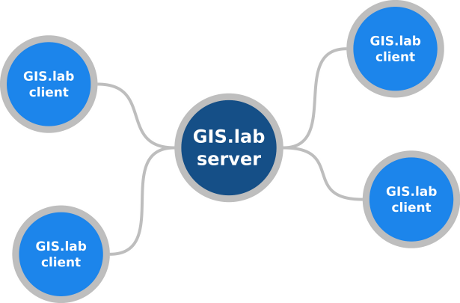
\includegraphics[width=.7\columnwidth]{figures/gislab-server-client-architecture.png}
  \caption{GIS.lab server-client based architecture (source: GIS.lab
    documentation)}
\label{fig:gislab_infrastructure}
\end{center}
\end{figure}

There is a large number of possible deployment scenarios in which
GIS.lab can be successfully used. GIS.lab can play a key role for
building geospatial computation cluster with effective horizontally
scalable computer power providing geospatial services to be consumed
by different clients within local network area or even in the data
center or cloud. GIS.lab is able to turn heterogeneous computers into
fully operative, centrally managed GIS easy-to-use system and
maintenance-free clients in few moments. It is ideal platform for GIS
\textit{education and popularization} of open source
technologies. GIS.lab technology is able to be incorporated into
existing computer network, or to create its own computer
network. Further option can be useful for crisis management in very
hard conditions of natural disaster with Internet outages. GIS.lab can
be customized in many ways in order to fulfill different requirements.

% KAO: Remove spacing before label: can cause reference to be wrong
\begin{figure}[ht!]
\begin{center}
  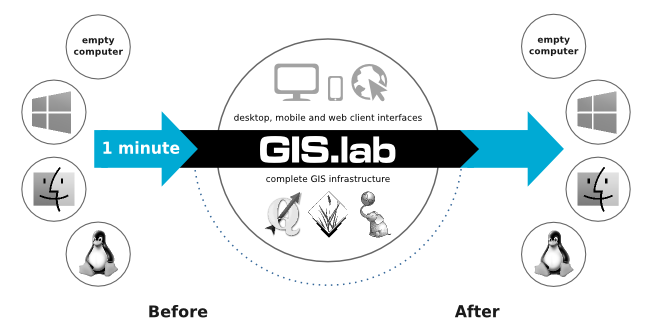
\includegraphics[width=1.0\columnwidth]{figures/gislab-architecture.png}
  \caption{GIS.lab infrastructure as a platform for teaching,
    computation, or crisis management (source: GIS.lab Documentation)}
\label{fig:gislab_infrastructure}
\end{center}
\end{figure}

This paper shows how to easily build complete open source GIS
infrastructure on the top of GIS.lab enabling highly specialized
hydrological modeling. Such system is performed by automated
customization of GIS.lab ecosystem including master (server) and
client nodes.

% KAO: Remove spacing before label: can cause reference to be wrong
\begin{figure}[ht!]
\begin{center}
  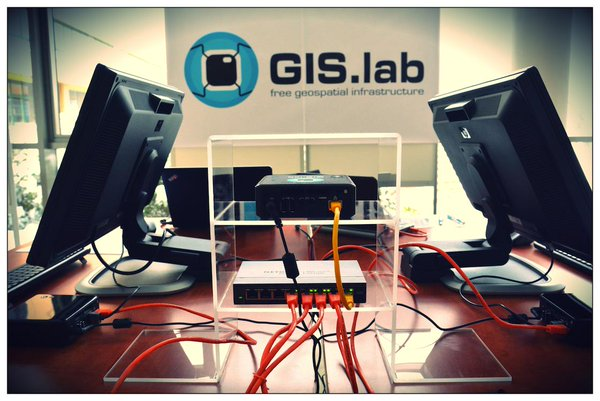
\includegraphics[width=0.9\columnwidth]{figures/gislab-real.jpg}
  \caption{GIS.lab components running in real environment (source:
    GIS.lab Documentation)}
\label{fig:gislab_infrastructure}
\end{center}
\end{figure}

\subsection{GIS Infrastructure for Hydrological Computation and
  Modeling}\label{GIS Infrastructure for Hydrological Computation and
  Modeling}

At first, let's put together basic requirements for presented
platform. Desired system should allowing the user to collect, prepare,
and preprocess data from heterogeneous data sources for hydrological
computation using GIS software packages. The user will be able to
perform hydrological computation locally on desktop clients, and also
consume dedicated geoprocessing service provided by a master node
running in the infrastructure. Results of hydrological modeling is
possible easily publish via web services from user desktop environment
and ideally also as interactive web mapping applications provided by
server component (master node) in the infrastructure.

Most of the requirements are already fulfilled by GIS.lab platform. It
provides fully established computer network consisting of server
(master node) and desktop clients (client nodes). GIS.lab main
objective is a rapid deployment of complete geospatial computation
platform enabling collaborative data managing, storing, processing,
analyzing thanks to fully automatic provisioning. On master node is
running Lighttpd web server in order to provide web services, PostGIS
geospatial database server to collect, store and manipulate with
geospatial data, GRASS GIS engine for performing geospatial analysis,
and QGIS Server providing OGC Web Services (OWS). On client side is
requested desktop GIS application to collect, manage and preprocess
input geospatial data. For this task GIS.lab desktop client offers
well known QGIS Desktop application. Performing hydrological modeling
in desktop environment can be possible thanks to integrated GRASS GIS
and QGIS GRASS plugin.

Missing features can be easily integrated into GIS.lab eco-system by
customization of deployment of the both master/server and desktop
client components. Since geoprocessing service should be provided by
the infrastructure the master node must be extended by application
able to provide OGC Web Processing Service (WPS). In this paper PyWPS
version 4 seamless deployment integration will be demonstrated.

Another missing component is a publishing platform providing ability
to easily publish results of computation in the form of an interactive
web mapping application. For this purpose will be used Gisquick open
source project. Gisquick integration will executed by using Docker
containers.

The last missing component -- a tool for hydrological modeling and
computation -- will be shown on GRASS AddOn tool
\textit{r.subdayprecip.design} integration in the sense of desktop
tool as well as a geoprocessing service implemented as OGC WPS
service. Presented \textit{r.subdayprecip.design} GRASS module
provides subday design precipitation totals based on hydrological
Hradek's method of reduction of daily maximums to chosen duration
\cite{landa.2015:FOSS4GE2015}.

\subsection{Gisquick as Publication Platform}

Gisquick (\url{http://gisquick.org}) is a separate project not
directly related to GIS.lab. It's web application based on modern
technologies like Django, Angular and OpenLayers 3 with fully
responsive design optimized also for mobile devices. The main purpose
of Gisquick is capability to easily publish QGIS projects on web. From
this perspective Gisquick is strongly connected to QGIS Desktop
environment and stands on QGIS Server component.

% KAO: Remove spacing before label: can cause reference to be wrong
\begin{figure}[ht!]
\begin{center}
  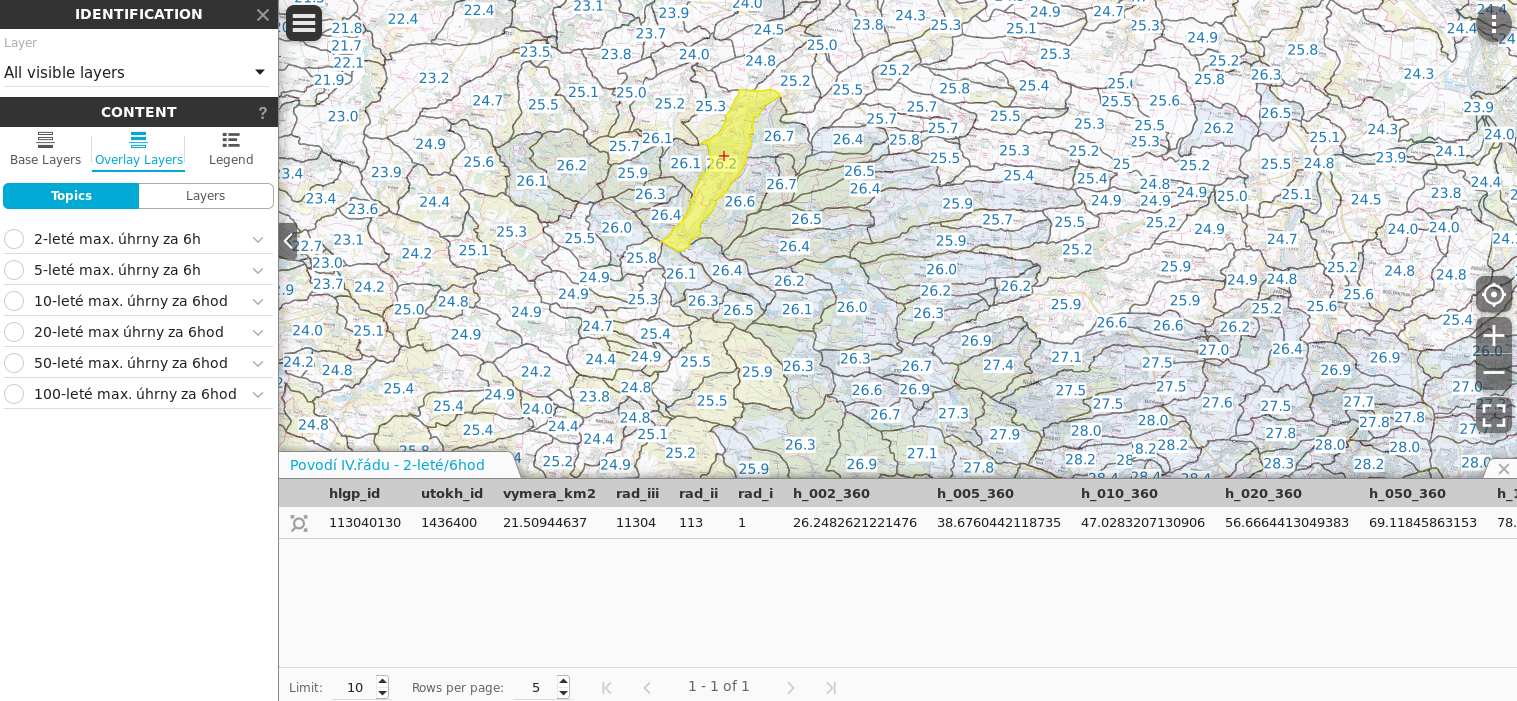
\includegraphics[width=0.9\columnwidth]{figures/gisquick-identify.png}
  \caption{Gisquick web application interface
    (source: author)}
\label{fig:gislab_infrastructure}
\end{center}
\end{figure}

Combining GIS.lab and Gisquick technologies leads to complete, seamlessly
integrated platform capable to prepare input data, perform geospatial
analysis and publish results easily on web in the sense of interactive
web mapping application.

\section{RAPID DEPLOYMENT OF CUSTOMIZED GEOSPATIAL CLUSTER}

\subsection{Fundamentals}

As mentioned earlier, one of the main objectives of GIS.lab technology
is a rapid and fully automated deployment. GIS.lab uses for this task
\textit{Ansible} framework. Ansible offers human-readable automatizing
language, agent-less execution, various modules and support for
different providers like AWS (Amazon Web Services), Azure and others
\cite{hochstein2014ansible}. It's important to mention that currently
GIS.lab (version 0.7) supports two providers: GIS.lab Unit and AWS. In
this paper we will focus on GIS.lab Unit provider in order to have
whole infrastructure under full control.

Described procedure consists of three major steps:

\begin{enumerate}
\setlength\itemsep{0em}\setlength\parskip{0em}\setlength\topsep{0em}\setlength\partopsep{0em}\setlength\parsep{0em}
\item{Deployment of master node using GIS.lab technology} 
\item{Master node customization}
\item{Gisquick integration}
\end{enumerate}

\subsection{Deployment of Master Node}\label{Deployment of Master Node}

Master node (playing a role of a server) of geospatial cluster can be
automatically deployed thanks to GIS.lab technology. There are some
hardware and software requirements which have to satisfied. First of
all, hardware on which the master node will be running need to be
available, it can be everything from Intel NUC unit (ideal for
testing) to real server rack hardware inhouse or provided by AWS,
Azure or similar services. The operator runs host (controlling)
machine which will be used for master node provision. On controlling
machine Ansible framework must be installed. Node(s) described in
so-called \textit{inventory} file are accessed over SSH.

% KAO: Remove spacing before label: can cause reference to be wrong
\begin{figure}[ht!]
\begin{center}
  
\includegraphics[width=0.9\columnwidth]{figures/gislab-unit.png}
  \caption{GIS.lab master node running on different providers (source:
    GIS.lab Documentation)}
\label{fig:gislab_infrastructure}
\end{center}
\end{figure}

At first on controlling machine needs to downloaded GIS.lab source
code (available freely from GitHub
repository\footnote{\url{https://github.com/gislab-npo/gislab}}) and
standard Ubuntu Server installation ISO image. In the next step a new
customized ISO will be created by GIS.lab utility
\texttt{gislab-unit-iso.sh} and used for installation on master node
hardware unit. After successful installation a plain Ubuntu operating
system will be available on that machine.

Afterwards two Ansible playbooks (both located in GIS.lab source code
tree) will be launched from the controlling machine. The first playbook
\texttt{gislab-unit.yml} is dedicated for Intel NUC only and stands
for GIS.lab Unit initialization. The second -- core -- playbook
\texttt{gislab.yml} performs provisioning whole GIS.lab technology on
master node equipment. It installs all required software packages, set
up all the services, creates and configure desktop client images. This
step can take from few dozen of minutes to few hours depending on Internet
connection speed and hardware limits. Simplified commands are shown
below.

\begin{lstlisting}
  $ ansible-playbook ... providers/../gislab-unit.yml
  $ ansible-playbook ... system/gislab.yml
\end{lstlisting}

% KAO: Remove spacing before label: can cause reference to be wrong
\begin{figure}[ht!]
\begin{center}
  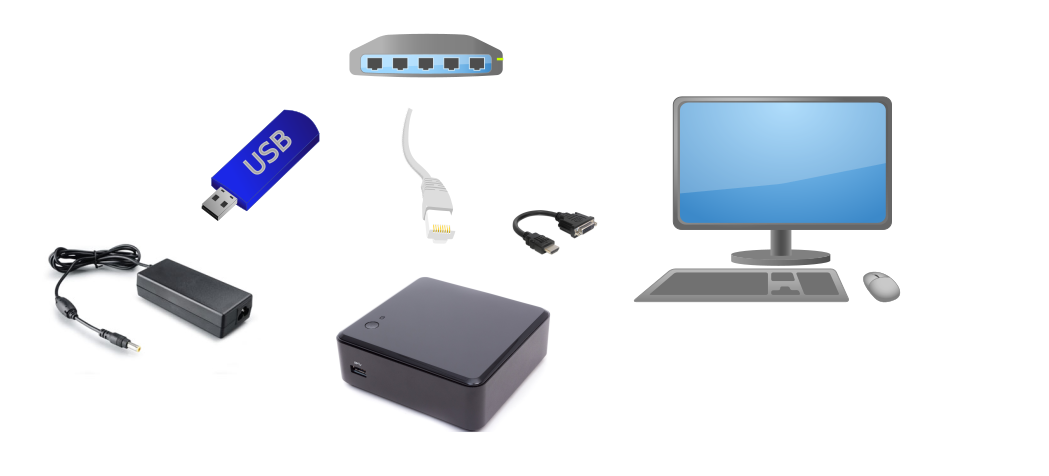
\includegraphics[width=1.0\columnwidth]{figures/installation-unit.png}
  \caption{All required hardware components for GIS.lab deployment
    (source: GIS.lab Documentation)}
\label{fig:gislab_infrastructure}
\end{center}
\end{figure}

Detail information about GIS.lab deployment procedure including its
configuration is part of an official GIS.lab documentation
\cite{gislab-docs}.

After successful deployment, a fully operative master node is running
in our infrastructure providing all the services which GIS.lab offers
out of the box. For our use-case is crucial database server
(PostgreSQL), map server (QGIS Server) and GIS computation engine
(GRASS GIS). All these components are available and configured by
GIS.lab. The clients can boot from master node using standard
protocols like PXE or HTTP. The master and clients node creating
geospatial cluster includes technologies like load balancing and
centrally managed system to control them. It also covers user accounts
management which is launched centrally by LDAP server running on
master node.

% KAO: Remove spacing before label: can cause reference to be wrong
\begin{figure}[ht!]
\begin{center}
  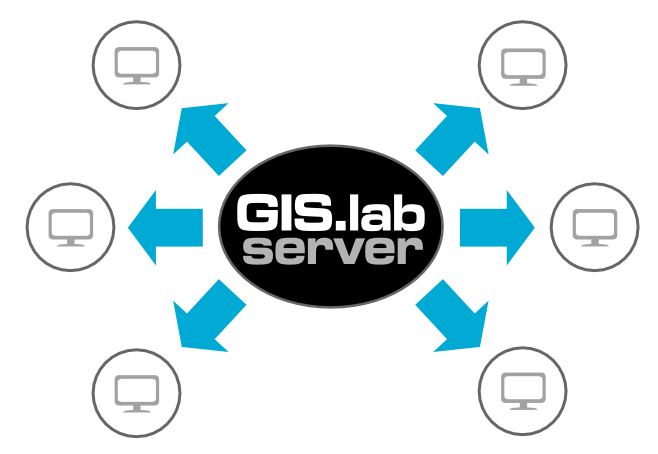
\includegraphics[width=1.0\columnwidth]{figures/gislab-machines-launch.png}
  \caption{Building geospatial cluster using master and client nodes
    (source: GIS.lab Documentation)}
\label{fig:gislab_infrastructure}
\end{center}
\end{figure}

\subsection{Master Node Customization}

Master node has been successfully deployed using GIS.lab
technology. In the following steps customization will be
performed. Customization rules are defined by \textit{Ansible
  Playbooks} similarly how GIS.lab provision works. Ansible Playbooks
express configurations, deployment, and orchestration in Ansible
\cite{shah2015ansible}. Playbooks are based on YAML human-readable
data serialization language and Jinja templates. As described in
section \ref{GIS Infrastructure for Hydrological Computation and
  Modeling} customization procedure will performed. Let's summarize
our requirements:

\begin{enumerate}
\setlength\itemsep{0em}\setlength\parskip{0em}\setlength\topsep{0em}\setlength\partopsep{0em}\setlength\parsep{0em}
\item{Install and configure PyWPS4 on GIS.lab master node}
\item{Install GRASS AddOn module \textit{r.subdayprecip.design} on
    server-side (master node) and also in client images in order to
    use this tool locally on desktop clients and also as remote
    geoprocessing service provided by PyWPS4 running on master node
    (server)}
\item{Set up PyWPS4 process based on \textit{r.subdayprecip.design}
  functionality.}
\end{enumerate}

Ansible Playbooks used for customization will be saved in
\textit{provision} directory and separated into set of
\textit{roles}. Each role is represented by \textit{tasks} which
perform calls to Ansible. Tasks for each role are defined in
\textit{main.yml} YAML file. Example below demonstrates how can be
implemented a role for installing and configuring PyPWS4.

\begin{lstlisting}[numbers=left,xleftmargin=1em]
- name: Install PyWPS4
  pip:
    name: pywps
    version: 4.0.0

- name: Set up PyWPS4 configuration
  template:
    src: pywps.cfg.j2
    dest: /opt/pywps4/pywps.cfg
    mode: 0644
\end{lstlisting}

PyWPS4 package will be installed by standard pythonic \textit{pip}
command which is implemented by Ansible \textit{pip module}, see lines
1-4. In the next step, PyWPS4 configuration file is placed in the
destination folder on the server, see lines 6-10. Simi\-larly is
processed PyWPS4 application file. From provisioning point of view,
the both files are placed in \textit{templates} directory. Template
module based on Jinja templating language allows variable
propagation. Simplified and shorten example of sample PyWPS4
configuration file \textit{pywps.cfg.j2} is shown below.

\begin{lstlisting}[numbers=left,xleftmargin=1em]
[server]
url={{ base_url }}/services/wps
\end{lstlisting}

Variable values can be defined in \textit{main.yml} file located in
\textit{vars} directory.

\begin{lstlisting}[numbers=left,xleftmargin=1em]
base_url: http://gislab.mydomain.org
\end{lstlisting}

In similar way will be defined other two roles for installing GRASS
tool \textit{r.subdayprecip.design} and related WPS process. The roles
are put together in main \textit{deployment.yml} YAML file.

\begin{lstlisting}[numbers=left,xleftmargin=1em]
roles:
    - { role: pywps4 }
    - { role: subdayprecip-tool }
    - { role: subdayprecip-wps }
\end{lstlisting}

Automated customization of master node will be perform by
\textit{Ansible Playbook} command similarly to GIS.lab deployment
procedure described in section \ref{Deployment of Master Node}.

\begin{lstlisting}
  $ ansible-playbook ... provision/deployment.yml
\end{lstlisting}

As a result of customization master node will be providing a new
service based on OGC WPS thanks to integrated PyWPS4 software
package. Newly installed GRASS tool providing hydrological computation
of subday design precipitation totals based on hydrological Hradek's
method of reduction of daily maximums to chosen duration will be
available on master node and desktop clients. Also ready-to-use WPS
process providing described functionality will be offered by master
node via OGC WPS service over HTTP(S) protocol.

Complete overview of customization Ansible Playbooks is available from
GitHub
repository\footnote{\url{https://github.com/ctu-geoforall-lab/subdayprecip-design}}. Another
example of GIS.lab customization is available from GISMentors training
group GitHub
repository\footnote{\url{https://github.com/GISMentors/gislab-customization}}.

\subsection{Gisquick integration}

On Gisquick publishing platform integration is demonstrated a
different approach. Instead of specific Ansible Playbooks, integration
based on \textit{Docker} containers will be performed. Gisquick
project provides core Docker images needed for successful running of
this publishing platform. It significantly simplifies Gisquick
integration into GIS.lab infrastructure.

The core Gisquick Dorker images are listed below:

\begin{itemize}
\setlength\itemsep{0em}\setlength\parskip{0em}\setlength\topsep{0em}\setlength\partopsep{0em}\setlength\parsep{0em}
\item{gisquick/nginx}
\item{gisquick/django}
\item{gisquick/qgisserver}
\end{itemize}

These Docker images can be automatically composed on GIS.lab master
node by running \textit{docker-compose} command.

\begin{lstlisting}
  $ sudo docker-compose up
\end{lstlisting}

This command need to be run in the directory where Dockerfile for
Gisquick are located. Official Dockerfiles are available from Gisquick
Git repository on
GitHub\footnote{\url{https://github.com/gislab-npo/gisquick}}. Before
running \textit{docker-compose} command a configuration rules for
composing Docker images must be created. The rules are stored in the
file named \textit{docker-compose.yml} located in the same directory
as Dockerfiles. Shorten example of compose YAML file is shown below.

\begin{lstlisting}[numbers=left,xleftmargin=1em]
version: "2"
services:
  qgisserver:
    image: gisquick/qgis-server
    volumes:
      - /storage/publish:/publish/:ro

  django:
    image: gisquick/django
    volumes:
      - /storage/media:/var/www/gisquick/media/
      - /storage/data:/var/www/gisquick/data/

  nginx:
    image: gisquick/nginx
    volumes:
      - /storage/letsencrypt/:/etc/letsencrypt/
\end{lstlisting}

The most important part of configuration from GIS.lab integration
point of view is definition of volumes, see lines 5, 10, 16. Here are
listed local directories which will be mounted into running Docker
containers. This procedure can be automized also Ansible Playbooks.

Gisquick is running on master node and it's available via HTTP(S)
protocol in the GIS.lab network. Clients can publish their projects by
QGIS Gisquick plugin and simply copying them to shared directories
mounted over NFS from master node(s).

\section{CONCLUSIONS}

Geospatial cluster can be arranged thanks to open source orchestration
technologies in automated and easy to maintain manner. This paper
presents Ansible framework allowing fully automatize software
provisioning, configuration management, and application deployment. On
the top of Ansible framework is built GIS.lab project. GIS.lab can
significantly simplifies whole procedure of designing, deploying and
configuring GIS infrastructure using centrally managed deployment to
absolute minimum. GIS.lab itself offers basic components, tools, and
services for building GIS (and not only GIS) infrastructure. GIS
cluster constists of master node and client nodes. Client nodes are
booting from master over PXE or HTTP boot protocols. Master node
services, user accounts, data volumes are centrally managed and
consumed by the clients over NFS (Network File System).

Master and client nodes can be customized using specific Ansible
Playbooks including software provisioning and also configuration
managent. Customized infrastructure can be easily deployed on new
hardware equipment. Integration of new compoments can be simplified by
using Docker containers in order to combining them into working system
seamlessly integrated into customized infrastructure.

{%\footnotesize
  \begin{spacing}{0.9}% tune the size by altering the parameter
    \bibliography{foss4g-eu-gislab-qisquick} 
  \end{spacing}
}

\section*{ACKNOWLEDGEMENTS}\label{ACKNOWLEDGEMENTS}

This work has been supported by the research project QJ1520265 -
"Variability of Short-term Precipitation and Runoff in Small Czech
Drainage Basins and its Influence on Water Resources Management".

The article is distributed under the Creative Commons Attribution 3.0
Unported License.

\end{document}
